\documentclass[11pt,a4paper]{jsarticle}
\usepackage[dvips]{graphicx}
\usepackage{fancyhdr}
\usepackage{here}
\setcounter{page}{0}
%
\begin{document}

\title{制御工学実験I \hspace{-0.1mm} I \hspace{-0.1mm} I \\ B2.台車の位置制御}
\author{提出者 \\ 14104064 下松八重 宏太 \\ \\ 共同実験者 \\ 14101028 梶野 翔平 \\ 14104092 中島 美香 \\ 16104311 北山 拓夢}
\date{同定実験日 2016年11月21日 \\ 計算実験日 2016年11月28日 \\ 制御実験
日 2016年12月5日 \\ 提出日 \today}



\maketitle
\thispagestyle{empty}
\newpage


\section{目的}
状態フィードバック制御を行うには全状態量をフィードバックする必要がある.しかしセンサの不足などによって実際に測定できない状態量が存在する場合には,オブザーバを用いて状態量を推定し,フィードバック制御に利用する.本実験では台車の位置制御実験を通じて,オブザーバによる状態フィードバック制御について理解を深める.

\section{原理}
  \subsection{数式モデル}
  モータの回転による力$T_u$を入力,台車の変位$y$を出力としたとき,運動方程式は次のようになる.
  \begin{equation}
   M\ddot{y}+F\ddot{y}=T_u
  \end{equation}
  $M$は台車の透過質量,$F$はレールと台車の間の摩擦係数である.$T_u$はパソコンからの指令電圧$u$に比例する.すなわち,$T_u = \alpha u$.ただし,$\alpha = 20.09$[N/V]. \\
  状態変数を$x = [x_1 x_2]^T = [y \dot{y}]$とおくと,次の状態方程式が得られる.
  \begin{eqnarray}
   \dot{x} &=& \left[
		\begin{array}{cc}
		 0 & 1 \\
		 0 & -\frac{F}{M}\\
		\end{array}
		  \right]
   + \left[
      \begin{array}{c}
       0 \\
       \frac{\alpha}{M}\\
      \end{array}
     \right]u \nonumber \\
   y &=& [1 \ 0]x
  \end{eqnarray}

  \subsection{未知パラメータの同定}
  状態フィードンバック制御系を構成するためには,式2の動特性パラメータがわかっている必要がある.システムのステップ応答より$F$と$M$を同定することが出来る.式2より,台車に一定の力を入力すると,台車は1方向に走り続ける.そこで,次の出力フィードバックをかける.
  \begin{equation}
   u = h(r-y)
  \end{equation}
  ここで,$r$は台車の目標変位,$h$はフィードバックゲイン定数である.すると,$r$から$y$までの伝達関数は次のようになる.また,この系の応答波形は$h$の値によって変わる.
  \begin{equation}
 G(s) = \frac{Y(s)}{R(s)} = \frac{b_0}{s^2+a_1 s +a_0} \ \ (a_1 = F/M,\ a_0 = b_0 = \alpha h/M)
  \end{equation}
  これより,$a_0,a_1$が求まれば,$F,M$が計算できる.ここで,2次遅れ系のステップ応答波形$y(t)$における最大行き過ぎ量$y_m$,行き過ぎ時間$t_m$,定常値$y_0$,を用いて次の式から$a_0,a_1$を求める.$y_m$は$t=0$以外で最初に$\dot{y(t) = 0}$となる時点$t_m$で生じていることを利用して,
  \begin{equation}
   a_1 = -\frac{1}{t_m}2\ln{(y_m/y_0 - 1)}, \ a_0 = \frac{\pi^2}{t_m^2} + \frac{a_1^2}{4}
  \end{equation}
  となる.また,$b_0 = a_0 y_0 /r$である.

  \subsection{同定結果の検証}  
  出力$y(t)$を求める.ステップ入力$r$のラプラス変換$R(s)=r/s$より,
  \begin{equation}
   Y(s) = \frac{b_0}{s^2+a_1 s +a_0}R(s) = \frac{\frac{y_0a_0}{r}}{s^2+a_1 s +a_0} \cdot \frac{r}{s} = \frac{a_0}{s^2+a_1 s +a_0} \cdot \frac{1}{s} \cdot y_0
  \end{equation}
  と表せる.ここで,
  \begin{equation}
   \frac{a_0}{s^2+a_1 s +a_0} = \frac{\omega_n^2}{s^2+2\xi \omega_n s +\omega_n^2}
  \end{equation}
  とおくと,
  \begin{equation}
   Y(s) = \frac{\omega_n^2}{s^2+2\xi \omega_n s +\omega_n^2}\cdot \frac{1}{s} \cdot y_0 
        = y_0 \left( \frac{1}{s} - \frac{s + 2\xi\omega_n^2}{s^2+2\xi \omega_n s +\omega_n^2} \right)
  \end{equation}
  となる.これを逆ラプラス変換して以下の式を求める.
  \begin{equation}
   y(t) = y_0 \left( 1-\frac{1}{\sqrt{1-\xi^2}}e^{-\beta t} \cos{(\gamma t-\delta)} \right)
  \end{equation}
  ただし,$\omega_n = \sqrt{a_0},\ \xi = \frac{a_1}{2\sqrt{a_0}},\ \beta = \xi \omega_n,\ \gamma = \omega_n \sqrt{1-\xi^2},\ \delta = \tan^{-1} \left(\frac{\xi}{\sqrt{1-\xi^2}} \right)$である.この同定結果に基づく時間応答と実験結果を比較し,同定パラメータが妥当か判断して必要なら修正する.

  \subsection{制御系の構成}
  式2に対して以下のように状態フィードバック制御系を構成する.
  \begin{eqnarray}
   \dot x(t) = {\bf Ax} (t) + {\bf b} u(t) \\
   y(t) = {\bf cx}(t)
  \end{eqnarray}
  ただし,
  \begin{eqnarray}
  {\bf A} = \left[
	    \begin{array}{cc}
	     0 & 1 \\
	     0 & -F/M \\
	    \end{array}
	   \right] \ 
  {\bf b} = \left[
	    \begin{array}{c}
	     0 \\
	     \alpha /M \\
	    \end{array}
	   \right] \ 
  {\bf c} = [1 \ 0] \\
   u(t) = - {\bf fx} (t) = [-f_1 \ -f_2][x_1(t) \ x_2(t)]^\mathrm{T}
  \end{eqnarray}
  本実験では,状態量{\bf x}(t)のうちセンサで検出できるのは台車位置$x_1(t)$のみであり,台車速度$x_2(t)$は検出できない.従って,状態フィードバック制御を行うにはオブザーバによる状態の推定量を用いる必要がある.そこで式11のプラントに対して,次の同一次元オブザーバを構成する.
  \begin{eqnarray}
   {\bf \dot{\hat{x}}}(t) &=& {\bf A} + {\bf b}u(t) + {\bf k}(y(t) - \hat y(t))\\
   \hat y(t) &=& {\bf \hat x}(t)
  \end{eqnarray}
  ${\bf \hat x}(t)$は状態${\bf x}(t)$の状態推定量である.これらより,台車を初期位置から目標位置に移動させる制御は次の入力を用いることで達成される.目標位置を$y_r$として,
  \begin{equation}
   u(t) = -{\bf f \hat x}(t) = -[f_1 \ -f_2][(\hat x_1(t) - y_r) \ \hat x_2(t)]^\mathrm{T}
  \end{equation}
  と表される.
 \section{実験方法}
  \subsection{同定実験}
  実験用のプログラムを用いて台車にステップ入力を入力する.ここで,目標ステップ変位$r=0.25$フィードバックゲイン$h = 10$とする.得られたデータより,台車のステップ応答波形を作成する.
 
 \subsection{計算実験}
 \begin{enumerate}
  \item 同定実験で得られたステップ応答波形より式4の$a_0,a_1$を求め,$F,M$を算出する.
  \item 求めたパラメータから式9より応答波形をシミュレーションし,同定実験結果と比較する.
  \item 状態フィードバック係数ベクトルを決める.
  \item オブザーバの各係数を計算する.
  \item 各パラメータが妥当か検討する.
 \end{enumerate}
ここで,プラントとオブザーバの係数を決めるためにそれぞれの伝達関数の極を求める.伝達関数の極を$\lambda_i = a_i + {\it j}b_i$とおくと極の実部$a_i$が負の時,出力波形は収束する.しかし,正の値のとき応答波形は発散する.

 \subsection{制御実験}
 ここでは式10,11で構成した状態フィードバック制御系によって台車を目標位置まで移動させる.プラントとオブザーバの極を変えて複数回実験を行い,結果をまとめる.
 
\section{実験結果}
  \subsection{同定実験}
  同定実験で得られた応答波形を図1に示す.図1より,最大行き過ぎ量$y_m = 0.327$[m],行き過ぎ時間$t_m = 0.55$[s],定常値$y_0 = 0.243$[m]とした.

  \begin{figure}[hb]
   \begin{center}
    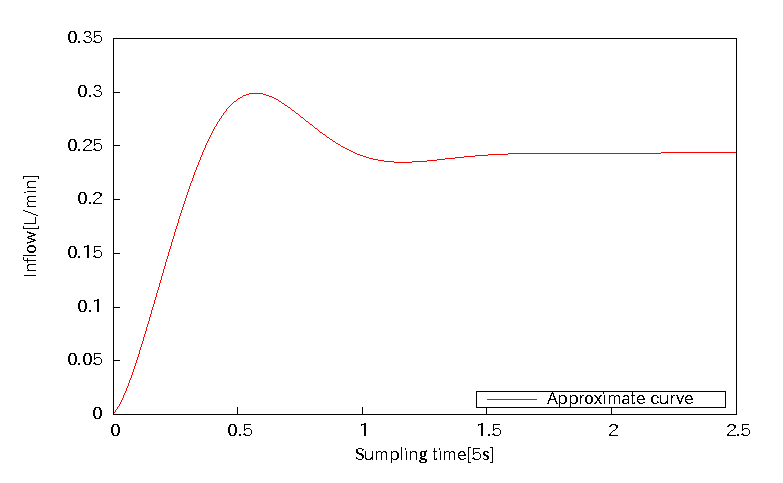
\includegraphics[scale=.8]{./picture/exp1.eps}
   \end{center}
   \caption{ステップ応答波形}
  \end{figure}
  
  \subsection{計算実験}
  同定実験結果より,
  \begin{equation}
   a_1 = 3.86, \ a_0 = 36.32
  \end{equation}
  と求まり,これより
  \begin{equation}
   F = 21.36, \ M = 5.53
  \end{equation}
  となった.求めた$a_0,a_1$を式9に代入し,このモデルの理論値を求めた.この理論値と実験値を比較するために,各時点での理論値と実験値の残差の和の絶対値ができるだけ最小となるように$a_0,a_1$を設定した.比較した結果を表1に示す.
  \begin{table}[b]
   \centering
   \caption{再設定した$a_0,a_1$と各時点での実験値との残差の和}
   \begin{tabular}{|c||c|c|c|} \hline 
    - & $a_0$ & $a_1$ & 残差の和 \\ \hline \hline
    理論値1 & 36.32 & 3.86 &  -0.07899 \\ \hline
    理論値2 & 36.3 & 3.8 & -0.07179 \\ \hline
    理論値3 & 36.5 & 3.7 & -0.05677 \\ \hline
    理論値4 & 36.6 & 3.605 & -0.04389 \\ \hline
   \end{tabular}
  \end{table}
  表1より,最も残差の和の絶対値が小さい理論値4を採用した.よって,$a_0 = 36.6,a_1 = 3.605$となり,これより$F \simeq 19.79,M \simeq 5.489$となった.
  
 \subsection{制御実験}
 プラントとオブザーバの極を変えつつ複数回実験を行った.結果を図2から図6に示す.プラントの極を$\Lambda_1 ,\lambda_2$,オブザーバの極を$\psi_1,\psi_2$とする.
 \newpage
 \begin{figure}[H]
  \begin{center}
   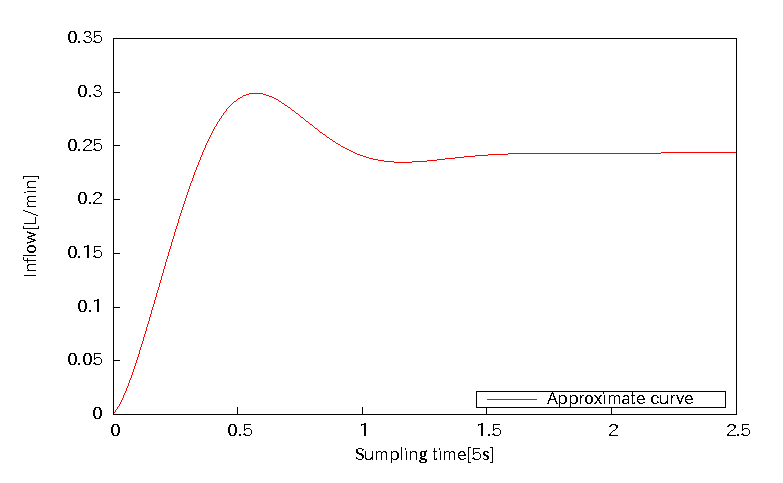
\includegraphics[scale = .8]{./picture/exp3.eps} \\
   (a) 台車位置と推定位置 \\
   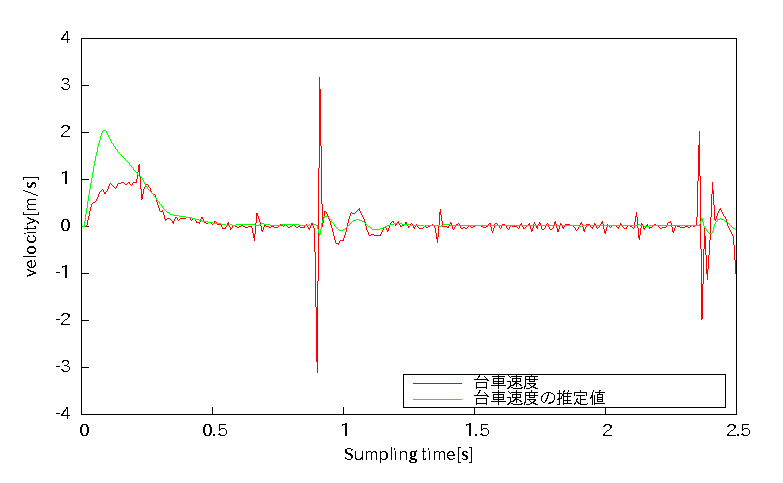
\includegraphics[scale = .8]{./picture/exp3_2.eps} \\
   (b) 台車速度と推定速度 \\
   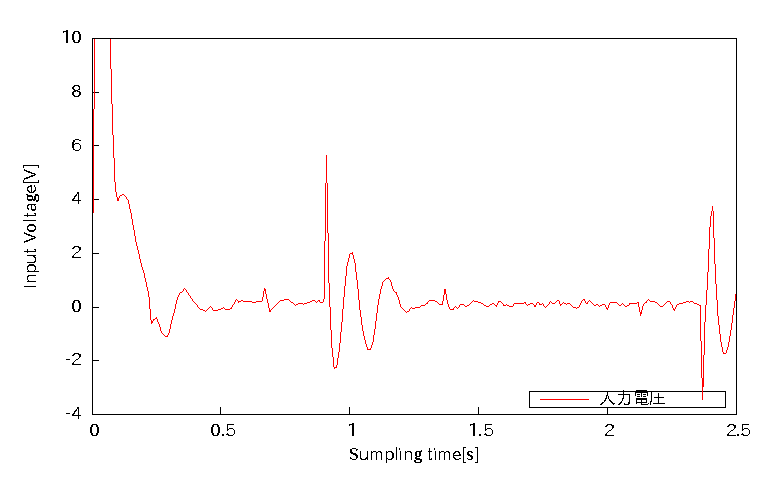
\includegraphics[scale = .8]{./picture/exp3_3.eps} \\
   (c) 入力電圧
  \end{center}
  \caption{$\lambda_1 = -20,\lambda_2 = -30, \psi_1 = -20,\psi_2 = -30$}
 \end{figure}

 \newpage
 \begin{figure}[H]
  \begin{center}
   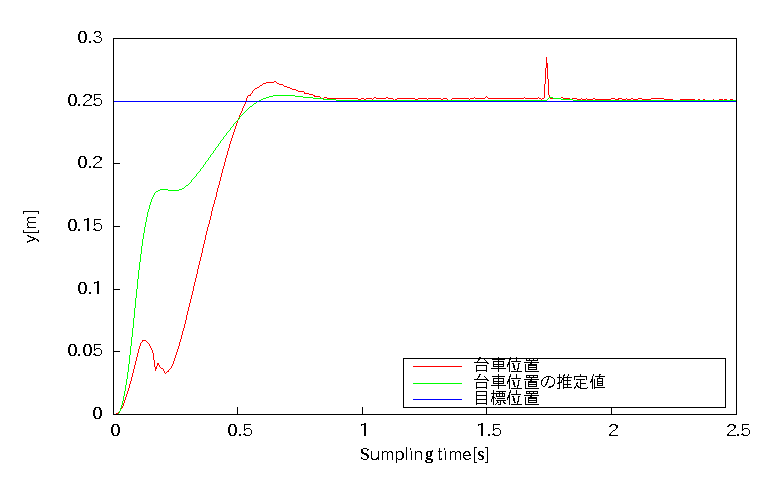
\includegraphics[scale = .8]{./picture/exp4.eps} \\
   (a) 台車位置と推定位置 \\
   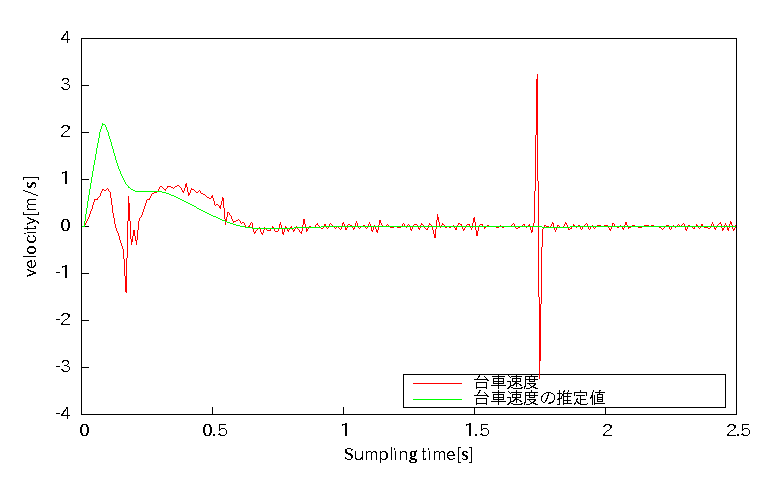
\includegraphics[scale = .8]{./picture/exp4_2.eps} \\
   (b) 台車速度と推定速度 \\
   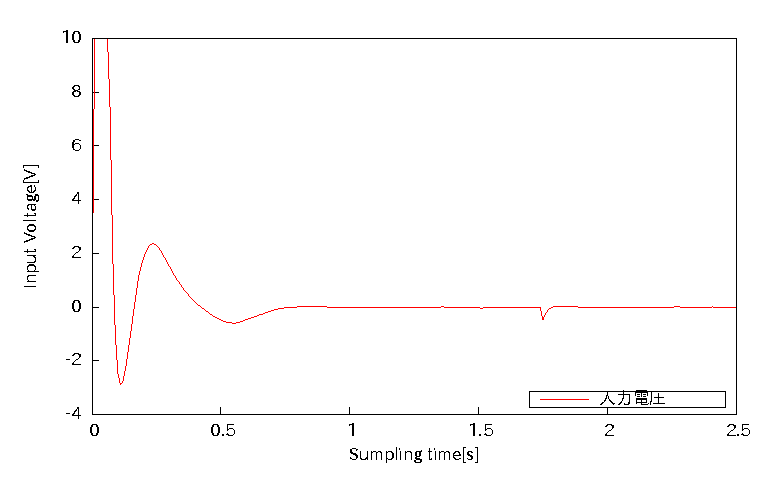
\includegraphics[scale = .8]{./picture/exp4_3.eps} \\
   (c) 入力電圧
  \end{center}
  \caption{$\lambda_1 = -20,\lambda_2 = -30, \psi_1 = -4,\psi_2 = -5$}
 \end{figure}

 \newpage
 \begin{figure}[H]
  \begin{center}
   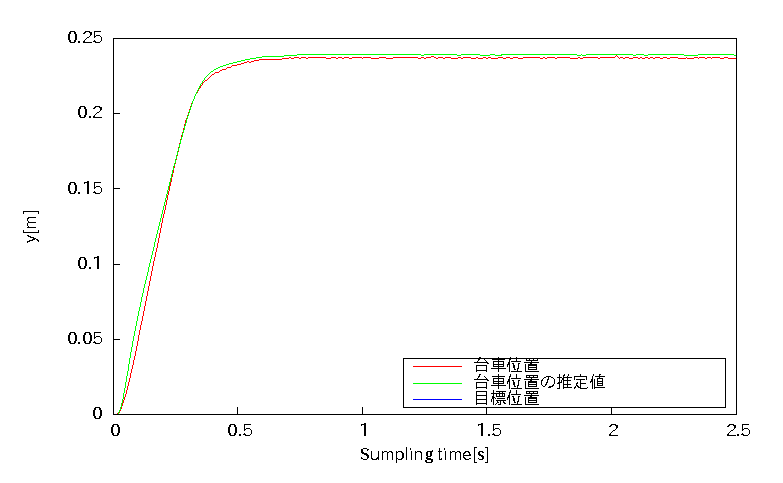
\includegraphics[scale = .8]{./picture/exp5.eps} \\
   (a) 台車位置と推定位置 \\
   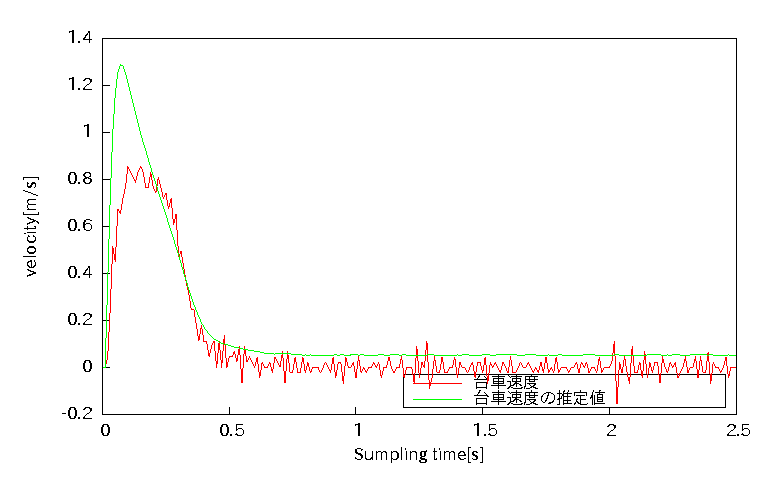
\includegraphics[scale = .8]{./picture/exp5_2.eps} \\
   (b) 台車速度と推定速度 \\
   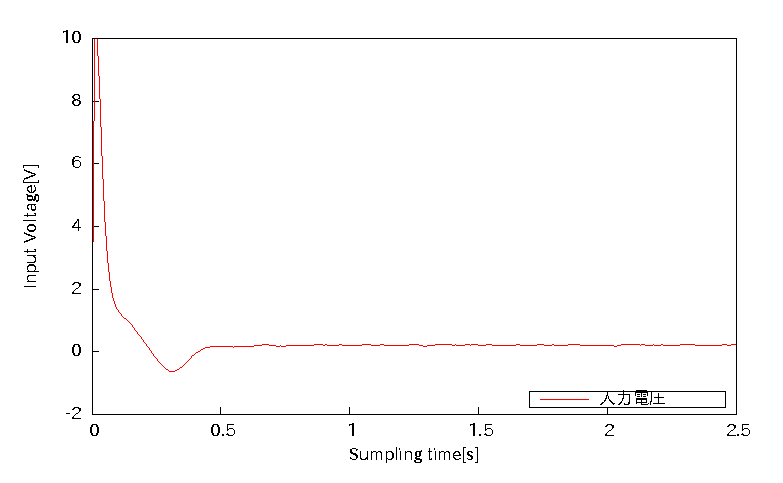
\includegraphics[scale = .8]{./picture/exp5_3.eps} \\
   (c) 入力電圧
  \end{center}
  \caption{$\lambda_1 = -10,\lambda_2 = -20, \psi_1 = -10,\psi_2 = -20$}
 \end{figure}

 \newpage
 \begin{figure}[H]
  \begin{center}
   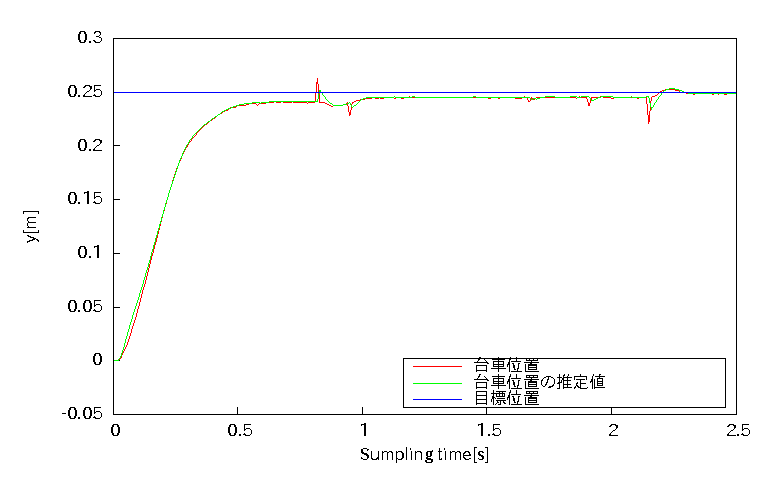
\includegraphics[scale = .8]{./picture/exp6.eps} \\
   (a) 台車位置と推定位置 \\
   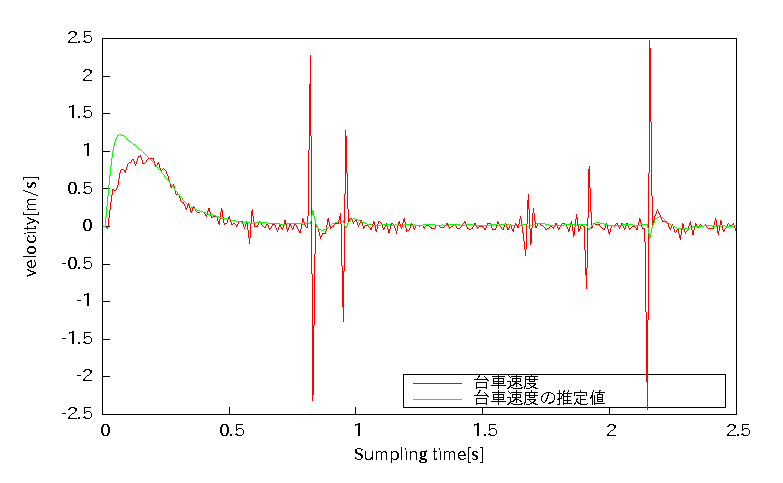
\includegraphics[scale = .8]{./picture/exp6_2.eps} \\
   (b) 台車速度と推定速度 \\
   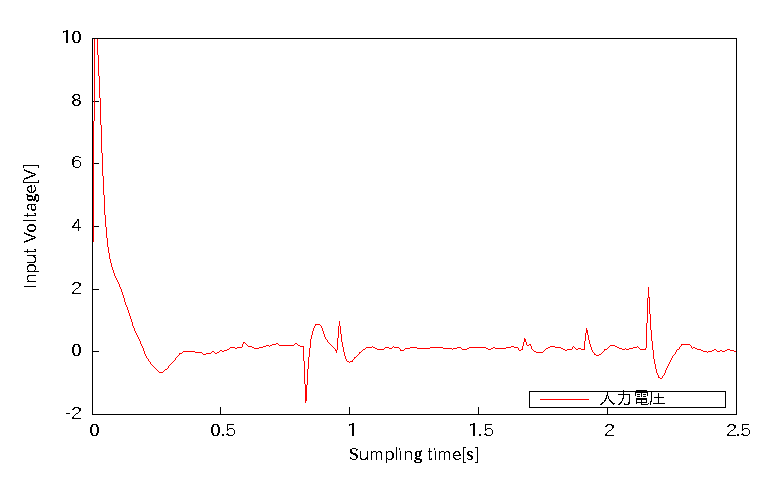
\includegraphics[scale = .8]{./picture/exp6_3.eps} \\
   (c) 入力電圧
  \end{center}
  \caption{$\lambda_1 = -10,\lambda_2 = -20, \psi_1 = -20,\psi_2 = -30$}
 \end{figure}

 \newpage
 \begin{figure}[H]
  \begin{center}
   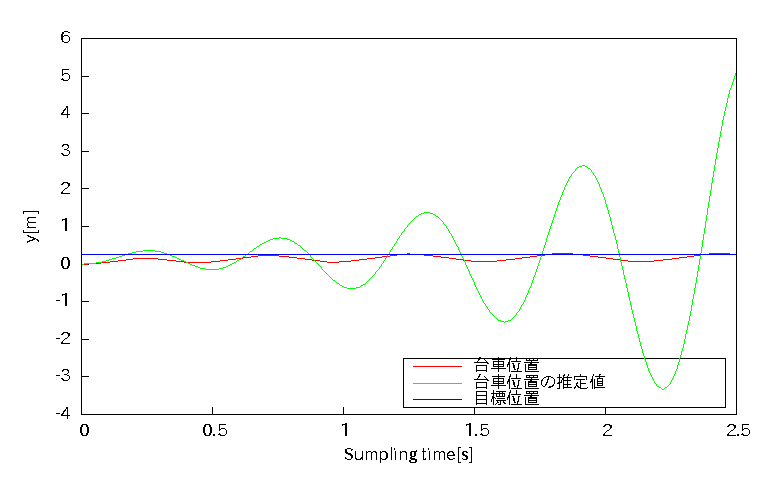
\includegraphics[scale = .8]{./picture/exp7.eps} \\
   (a) 台車位置と推定位置 \\
   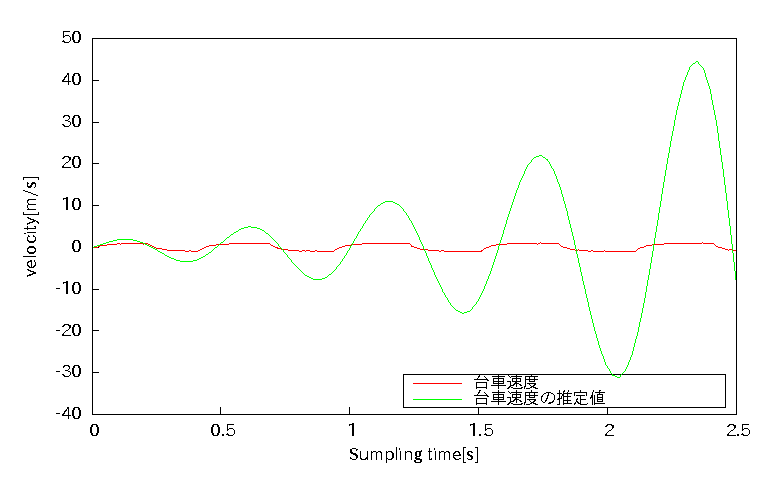
\includegraphics[scale = .8]{./picture/exp7_2.eps} \\
   (b) 台車速度と推定速度 \\
   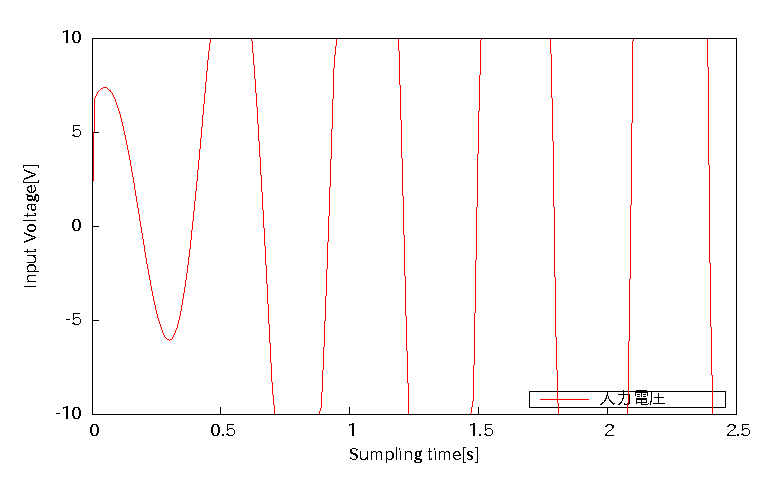
\includegraphics[scale = .8]{./picture/exp7_3.eps} \\
   (c) 入力電圧
  \end{center}
  \caption{$\lambda_1 = -10{\it j},\lambda_2 = 10{\it j}, \psi_1 = -10{\it j},\psi_2 = 10{\it j}$}
 \end{figure}

\newpage
 \section{考察}
  \subsection{プラントとオブザーバの極について}
  まず,図2の時のそれぞれの極は実験中比較的早く定常状態になった極である.ここからプラントとオブザーバの極の大小関係を変化させたところ,図3のようになった.図2と比較すると,オーバーシュートが生じていることがわかる.次にそれぞれの極を大きくしてみたところ,図4のようになった.図2と比較すると定常状態での目標位置との差が大きいがより早く定常状態に達している.次にオブザーバの極を小さくしてみたところ,図4と比べて目標位置との差が小さい.最後に図5はそれぞれの極の実部を0として,虚部のみにした場合の結果である.このとき,応答波形は振動していることがわかる.\\
  また,それぞれの速度のグラフにおいて大きく振動している部分があるが,これは速度を実際に計測しておらず,エンコーダの位置情報から速度を算出しているためである.それに伴い,入力電圧も振動している.


\newpage
\section{課題}
\subsection{併合系の状態方程式}
併合系とはレギュレータとオブザーバの状態方程式を併合した系である.
\begin{equation}
 z = (x_1 \ x_2 \ \hat x_1 \ \hat x_2)^\mathrm{T} 
\end{equation}
とおくと,式10,14より
\begin{eqnarray*}
 {\bf \dot x = Ax + b}u \\
 {\bf \dot{\hat x} = kcx + (A - kc)\hat x + b}u \\
\end{eqnarray*}
となるので,
\begin{eqnarray}
 {\bf \dot z} & = & {\bf(\dot x \ \dot{\hat x})^\mathrm{T}} \nonumber \\
             & = & \left(\begin{array}{cc}
		          {\bf A} & 0\\
			  {\bf kc} & {\bf A-kc} \\
			 \end{array}\right){\bf z}
	     + \left(\begin{array}{c}
		{\bf b}\\
		{\bf b}\\
		     \end{array}\right) u
\end{eqnarray}
と表せる.
式20より,特性方程式が求まり,レギュレータ及びオブザーバの極を設定出来る.
\subsection{制御系のパラメータについて}
一般的に線形系の状態フィードバック制御における安定性と応答の早さは固有値の実数部によって支配されている.固有値全てを複素平面上の左半面のできるだけ左側に持っていくことが出来れば,系は安定で応答も早くなるはずである.系が可制御のとき,常に状態フィードバックによる極配置は可能である.オブザーバを用いた状態フィードバック制御の場合,状態値と推定値の誤差が0に収束するように式20における$k$を選ぶ.

\begin{thebibliography}{1}
 \bibitem{1} 嘉納 英明,``現代制御工学-動的システムの解析と制御-'',日刊工業新聞社,1984,pp.161-164,179.
\end{thebibliography}

\newpage
\setcounter{page}{1}
\setcounter{section}{4}
%\renewcommand{\thepage}{\thepage}
\pagestyle{fancy}
\renewcommand{\headrulewidth}{0.0pt}
\rhead{再\thepage}
\lhead{}
\cfoot{}

\section{実験結果}

\end{document}



 




